\documentclass[USenglish,oneside,twocolumn]{article}
\usepackage{color}
\usepackage[hyphens]{url}
\usepackage{longtable}
\usepackage{graphicx}
\usepackage{enumitem}
\usepackage{pdfpages}
\usepackage{adjustbox}
\usepackage{subcaption}
%\usepackage{hyperref}

\usepackage[utf8]{inputenc}%(only for the pdftex engine)
%\RequirePackage[no-math]{fontspec}%(only for the luatex or the xetex engine)
\usepackage[big]{dgruyter_NEW}
 
\hyphenation{Isa-bela}

\DOI{foobar}

\cclogo{
\includegraphics{by-nc-nd.pdf}}

% Format a participant quotation.
\newcommand{\pquote}[2]{
\begin{quotation}
\noindent #1:~\textit{#2}
\end{quotation}
}
  
\begin{document}
   \author*[1]{Author 1}

  \author[2]{Author 2}

  \author[3]{Author 3}

  \author[4]{Author 4}

  \author[5]{Author 5}
  
  \author[6]{Author 6}

  \affil[1]{Affiliation of Author 1, E-mail: \mbox{author1@affiliation.edu}}
  \affil[2]{Affiliation of Author 2, E-mail: \mbox{author2@affiliation.edu}}
  \affil[3]{Affiliation of Author 3, E-mail: \mbox{author3@affiliation.edu}}
  \affil[4]{Affiliation of Author 4, E-mail: \mbox{author4@affiliation.edu}}
  \affil[5]{Affiliation of Author 5, E-mail: \mbox{author5@affiliation.edu}}
  \affil[6]{Affiliation of Author 6, E-mail: \mbox{author6@affiliation.edu}}
%  \author*[1]{Linda Lee}
%
%  \author[2]{David Fifield}
%
%  \author[3]{Nathan Malkin}
%
%  \author[4]{Ganesh Iyer}
%
%  \author[5]{Serge Egelman}
%  
%  \author[6]{David Wagner}
%
%  \affil[1]{University of California Berkeley, E-mail: \mbox{lnl@cs.berkeley.edu}}
%
%  \affil[2]{University of California Berkeley, E-mail: \mbox{fifield@cs.berkeley.edu}}
%
%  \affil[3]{University of California Berkeley, E-mail: \mbox{nmalkin@cs.berkeley.edu}}
%
%  \affil[4]{University of California Berkeley, E-mail: \mbox{ganesh.v@berkeley.edu}}
%  
%  \affil[5]{University of California Berkeley and International Computer Science Institute, E-mail: \mbox{egelman@cs.berkeley.edu}}
%   
%  \affil[6]{University of California Berkeley, E-mail: \mbox{daw@cs.berkeley.edu}}

  \title{\huge A Usability Evaluation of Tor Launcher}

  \runningtitle{A Usability Evaluation of Tor Launcher}

  %\subtitle{...}

  \begin{abstract}
{
We perform the first usability test on Tor Launcher, a graphical user interface (GUI) 
that all Tor Browser users must use to configure their initial connection to the Tor network. 
We believe that the interface is usable if a new user can to identify what to do,
knows if and when they do the right thing in the process, 
and configures the necessary network components to connect to Tor. 
We use a combination of user observations and user interaction logs to determine
where the interface is not usable, and quantify how unusable the interface is. We 
offer some suggestions for the interface based on what 
we have learned and also suggest alternative approaches 
to bootstrap a connection to Tor that do not require new users to configure the network components. 
}
\end{abstract}
  \keywords{Usable Security, User Studies, Tor, Security, Censorship, Anonymity}
%  \classification[PACS]{}
 % \communicated{...}
 % \dedication{...}

  \journalname{Proceedings on Privacy Enhancing Technologies}
\DOI{Editor to enter DOI}
  \startpage{1}
  \received{..}
  \revised{..}
  \accepted{..}

  \journalyear{2015}
  \journalvolume{2015}
  \journalissue{2}

\maketitle

\section{Introduction}

Tor~\cite{dingledine2004tor} is an anonymity network that routes Internet traffic through a series of relays 
that make it difficult to observe the source and destination. 
Tor Browser~\cite{torbrowser} is a modified Firefox browser with a built-in Tor client that
is the recommended way to use Tor. Tor Launcher is a Tor Browser component that
starts, stops, and otherwise controls the underlying Tor processes.
Tor Launcher's graphical user interface asks the user to configure
bridges, pluggable transports, and proxies to make a connection to Tor (we refer to this graphical user interface as the ``configuration interface'' throughout this paper). This is the object of our study. 

Although Tor Browser was originally designed for Internet anonymity, many now use Tor Browser to circumvent Internet censorship. In fact, many countries block Tor relays specifically to prevent their citizens from circumventing censorship~\cite{winter2012great}. The configuration interface mainly exists so that people who face Internet censorship can configure bridges, transports, and proxies to connect to Tor, but all Tor Browser users must interact with it regardless of why they use Tor Browser.

Tor minimizes collecting user data. Therefore, Tor does not have data on how users interact with the configuration interface. While we agree that this is respectful to the users, we also believe that this data will be helpful to improve the usability of the configuration interface. Improving the usability of the configuration interface has the obvious benefit of helping more users connect to Tor. But this is also benefits the Tor company (less help desk tickets) and other Tor users (an increase in overall users increases the anonymity set~\cite{dingledine2006anonymity}). 

We started our usability evaluation by inspecting the interface (section~\ref{sec:inspection}) and
running observing participants interact with it (section~\ref{sec:qualitative}). 
We opportunistically used the insights from our observations to make some changes (section~\ref{sec:design}).
Then we quantified how usable the interface was, and 
how much our changes helped save users time (section~\ref{sec:quantitative}).
Afterward, we gave some recommendations (section~\ref{sec:recommendations}), addressed
limitations of our evaluation (section~\ref{sec:limitations}), and framed our work in the context of existing work (section~\ref{sec:related}). \\

\noindent This paper contributes:
\smallskip
\begin{itemize}
\item an inspection of the Tor Launcher 5.0.3 interface
\item user connection attempts in various environments
\item what users found challenging about the interface
\item measurements of how many users could connect
\item measurements of how long users took to connect
\item patterns seen in the users that failed to connect
\item recommendations to improve the interface
\item alternatives to burdening users with configuration 
\end{itemize}

\section{Background}
\label{sec:background}
This section covers technical background necessary to understand the study. 

\subsection{Relays, Bridges, Pluggable Transports, and Proxies} 

Tor relays are routers in the Tor Network that receive and route Tor traffic. 
The three types of relays are: guard relays that serve as an entry node, middle relays that forward traffic from an entry relay to an exit relay, and exit relays which direct traffic to the destination. 

Bridges are unlisted Tor relays that serve as an alternative entry node.
Bridges can be unlisted relays that behave similarly to a regular Tor relay,  
but most run a pluggable transport (referred to as ``transport'' for shorthand) that obfuscates traffic. 
Most transports rely on the secrecy of their static IP addresses for their effectiveness.
These include ``fte'' and ``fte-ipv6''~\cite{fte},
which disguise the Tor protocol as another protocol (such as HTTP), and
``obfs3''~\cite{obfs3}, ``obfs4''~\cite{obfs4}, and ``scramblesuit''~\cite{scramblesuit},
which encrypt or alter the Tor protocol to appear as random noise.
Other transports route traffic through other services and do not need secret IP address. 
``flashproxy''~\cite{flashproxy} connects through third party web browsers,
and the ``meek''~\cite{fifield2015blocking} options route traffic
through content delivery networks. Fig.~\ref{fig:bridge-options} shows the bridge and transport options at the time of the study.

\begin{figure}
  \centering
    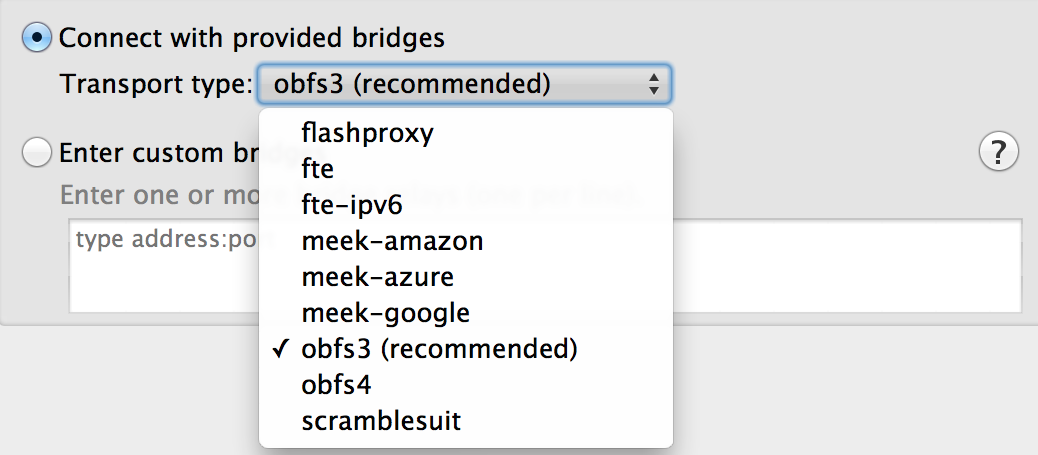
\includegraphics[width=0.5\textwidth]{bridge-options.png}
\caption{
Bridge options in Tor Browser~5.0.3's Tor Launcher interface.
Pre-configured bridges can be selected by ``Transport type,'' which refer to various
censorship circumvention technologies (``pluggable transports'').
%Under ``Enter custom bridges,'' there is a space to paste in
%a bridge line, obtained out of band.
%The ``Help'' button displays instructions on obtaining
%bridge lines. 
}
\label{fig:bridge-options}
\end{figure}

In this paper, ``proxy'' refers to a local, ordinary unobfuscated proxy such as a SOCKS or HTTP proxy. (Technically, Tor relays, bridges, and local proxies all allow indirect network connections to other network services and can be considered a proxy.) Fig.~\ref{fig:topology} illustrates the interacting components.

\begin{figure}
\centering

\includegraphics{topology.pdf}
\caption{
The chain of components involved in connecting to a website over Tor.
Most users do not need a proxy;
only users who face a censor need a bridge.
In the diagram, ``Tor'' represents all three anonymizing hops through the Tor network.
We have shown the bridge as a separate component
because of the special role it plays.
When a bridge is used, it becomes the first Tor relay.
}
\label{fig:topology}
\end{figure}

\subsection{State and Corporate Censorship}
State level censors block access to the Tor network by blocking Tor relays, which are publicly listed. Some also employ more sophisticated techniques such as deep packet inspection and protocol detection. This means that users can connect to the Internet, but not through Tor. The thoroughness of censorship is what requires different bridges and transports. 

A local proxy is required to connect in certain managed networks (i.e. company and university firewalls). This usually means that users cannot connect to the Internet at all without a proxy, including connecting to the Internet through Tor. The user must be able to connect to the Internet through their proxy before trying to connect to the Internet with Tor. 

\subsection{Connecting to Tor} 
Configuring a bridge requires providing one or more
``bridge lines,'' a specifically formatted bridge specification that
includes its IP address, transport type, and other metadata.
The interface has hard-coded options (see Figure~\ref{fig:bridge-options}) 
that select a group of bridges that use a particular transport.
For instance, choosing the hard-coded obfs3 option
configures a handful of bridges that use obfs3 transport.
If the built-in bridges do not work, a user can obtain bridge lines
through out-of-band channels, for instance by email~\cite{bridgedb}.

Configuring a proxy requires providing the proxy protocol, IP address, port, and additional optional fields. The user must locate and input this information. If the computer is already configured to use a proxy, the information can be found in other browsers. The interface tells users to ``check Internet settings in another browser'' if they are unsure of the proxy information. 

There are many valid configuration settings to connect to the Tor network.
A user who needs a bridge can connect to Tor with a bridge and proxy, provided that both were configured correctly.

\section{Methodology} 
This section discusses our process, principles, and preparations for evaluating the configuration interface.

\subsection{Testing Pipeline} 
Two researchers first performed a cognitive walkthrough~\cite{cognitive-walkthrough} to prepare for user testing. A cognitive walkthrough is evaluation method that requires usability evaluators to work through a series of tasks from the perspective of the user, usually to understand a system's learnability for new or infrequent users.

We then conducted a formative usability test~\cite{formative} that found where and why users struggle. This testing is usually used as a support tool to find improvements. Five users is considered to be the maximum benefit-cost ratio for gaining insights~\cite{howmanyusers}, so we recruited five participants for each experimental condition. 

We opportunistically used our observations to make changes to the interface. We believed that the process of identifying design principles, drafting design changes, and testing an alternative interface would be insightful and have the potential to discover impactful changes.

We concluded with a summative usability test~\cite{summative} that measured the usability of the current and redesigned interface. This testing is a usually used as quality assurance tool to test features. In short, formative testing tells you {\it what} is is not usable, while summative testing testing tells you {\it if} it is or is not usable. Twenty users is considered to be a minimum for statistically significant measurements~\cite{howmanyusers}, so we recruited twenty participants for each experimental condition.  

\subsection{Evaluation Metrics}
\label{sec:eval}
Usability measures users' abilities to complete tasks. We use the following industry-standard~\cite{albert2013measuring} metrics: \\

\begin{itemize}
\item {\bfseries Completion rate:}  percentage of users that connect to Tor in an experimental condition. 
\item {\bfseries Connection time:} time from Tor Browser startup to a successful connection to Tor. 
\item {\bfseries Configuration time:} time users spent in Tor Launcher configuring bridges and proxies.
\end{itemize}

Completion rate is the fundamental usability metric that measures if users can accomplish the task. We defined success as a binary metric that is true if a user connected to Tor and false if a user did not. 

Task time is a supplemental usability metric that measures user productivity during the task. We measured task time two different ways. Connection time measures how long users use the configuration interface, which includes time  spent waiting while a Tor Browser establishes a connection to Tor, which can dominate the measurement. Configuration time measures the time users spent actively configuring bridges and proxies. 

\subsection{Experimental Setup}
\label{sec:environments}
We use versions of Tor Browser~5.0.3, 
the most recent stable release at the time~\cite{torbrowser-503}.
There were new releases during the experiments, but
we used the same version throughout to not introduce
confounding factors.

We simulated three environments of increasing severity in censorship (E1, E2, E3).
Table~\ref{tab:environments} summarizes them and explains what is required to connect to Tor. We chose to 
simulate environments for the stability and reproducibility of the 
experiment, as real censored networks are volatile and complex. 

\begin{table}[t]
\centering
\begin{tabular}{r c c c}
& E1 & E2 & E3 \\
% \noalign{\hrule}
websites blocked & X & X & X \\
public relays blocked & & X & X \\
default bridges blocked & & & X \\
\end{tabular}
\caption{
Summary of our simulated censorship environments.
E1 only requires users to connect directly;
E2 requires users to connect with a built-in bridge;
and E3 requires users to connect with a specific type of built-in bridge
or a custom bridge.
E2's blocking is a superset of E1's;
similarly E3's is a superset of E2's.
}
\label{tab:environments}
\end{table}

The simulated environments are not intended to imitate any particular country's censorship environment. Rather, they were designed to require particular network configurations
to connect to Tor. We believe this to be sufficient for the purpose of testing the configuration interface, since these environments require the user to take the interface paths we wanted to test. 

We used Windows Firewall rules to block IP address of public Tor relays (E2, E3) and default bridges (E3). 
We used the Windows operating system hosts file to to block websites by
mapping domain names to localhost (127.0.0.1) (E1, E2, E3). We blocked torproject.org and its subdomains to discourage downloading Tor Browser, as we had installed a specific version on the test computers.  We blocked wikipedia.org, cnn.com, and their subdomains to create ``censored'' sites for the experiment. 

\section{Usability Inspection}
\label{sec:inspection}
This section discusses our inspection of the configuration interface and the resulting observations.

\subsection{Procedure} 
Two researchers performed the cognitive walkthrough on the Tor Browser 5.0.3 Tor Launcher GUI, the most recent version deployed at the time (Figure~\ref{fig:old-interface}). We systematically tried action sequences from the perspective of a typical user, which we defined as a first time or infrequent user with almost no previous knowledge about network components involved in connecting to Tor.

We first examined each screen in the interface for tasks required, inputs taken, and consequences of possible actions. This was done to map all potential paths through the interface (Figure~\ref{fig:digraph}). We then stepped through each user path and recorded our observations. 

\begin{figure*}
\centering
\begin{subfigure}[b]{0.35\textwidth}
	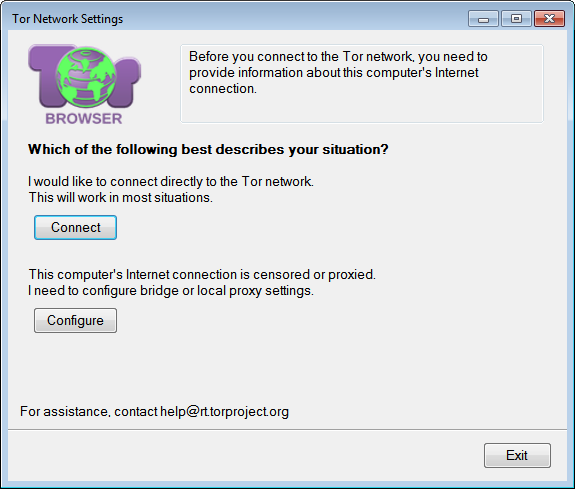
\includegraphics[width=\textwidth]{screenshots/OLD-first.png}
	\caption{The first screen. The connect button does not connect directly, but uses settings configured in the interface (initialized to be direct).}
	\label{fig:old-first}
\end{subfigure}
~~~~~~~~~~
\begin{subfigure}[b]{0.35\textwidth}
	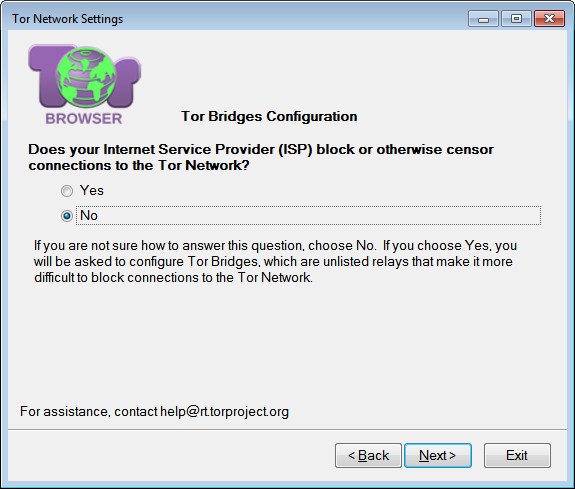
\includegraphics[width=\textwidth]{screenshots/OLD-bridges.png}
	\caption{Answering yes to this question leads to a screen to configure bridges. Answering no leads to the proxy question screen (Figure~\ref{fig:old-proxy}).}
	\label{fig:old-bridge}
\end{subfigure}
\begin{subfigure}[b]{0.35\textwidth}
	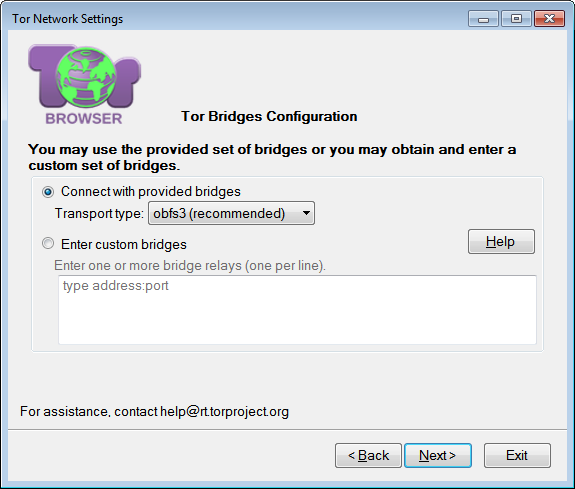
\includegraphics[width=\textwidth]{screenshots/OLD-bridgeSettings.png}
	\caption{Where users choose a bridge. The recommended bridge is a hard-coded obfs3.}
	\label{fig:old-bridge-settings}
\end{subfigure}
~~~~~~~~~~
\begin{subfigure}[b]{0.35\textwidth}
	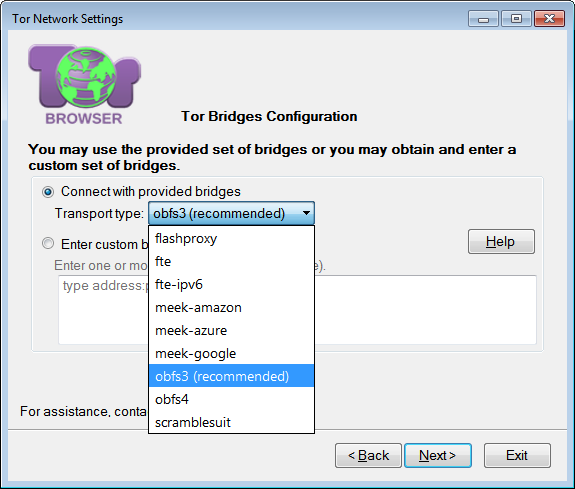
\includegraphics[width=\textwidth]{screenshots/OLD-bridgeSettings-combobox.png}
	\caption{The available transport selections, listed in alphabetical order. They all work differently.}
	\label{fig:old-bridge-combobox}
\end{subfigure}
\begin{subfigure}[b]{0.35\textwidth}
	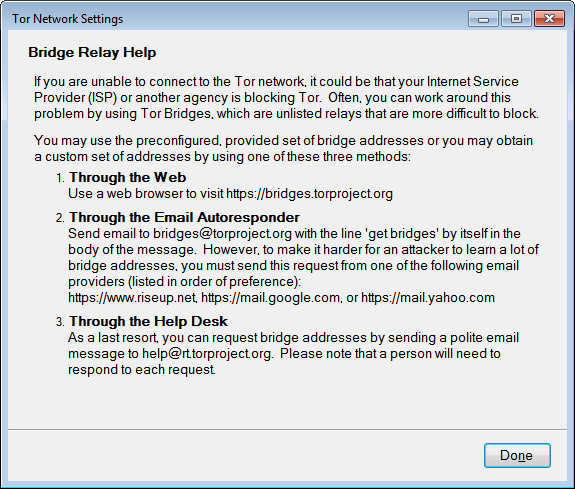
\includegraphics[width=\textwidth]{screenshots/OLD-bridgeHelp.png}
	\caption{Instructions on getting a custom bridge.Clicking the ``Help'' button in Figures~\ref{fig:old-bridge-settings} and \ref {fig:old-bridge-combobox} leads to this page.}
	\label{fig:old-bridge-help}
\end{subfigure}
~~~~~~~~~~
\begin{subfigure}[b]{0.35\textwidth}
	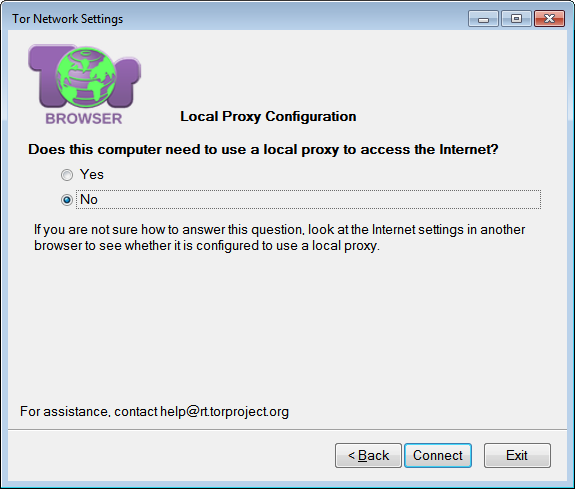
\includegraphics[width=\textwidth]{screenshots/OLD-proxy.png}
	\caption{Answering yes to this question leads to a screen to configure proxies. Answering no initiates a connection to Tor.}
	\label{fig:old-proxy}
\end{subfigure}
\begin{subfigure}[b]{0.35\textwidth}
	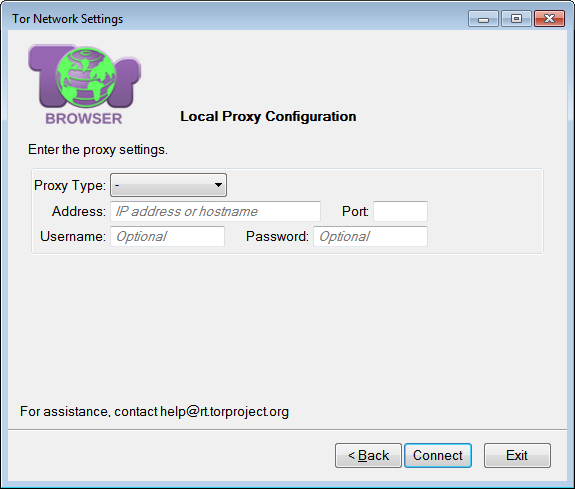
\includegraphics[width=\textwidth]{screenshots/OLD-proxyYES.png}
	\caption{Where users fill in proxy information.}
	\label{fig:old-proxy-yes}
\end{subfigure}
~~~~~~~~~~
\begin{subfigure}[b]{0.35\textwidth}
	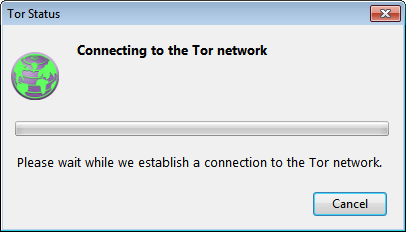
\includegraphics[width=\textwidth]{screenshots/OLD-progress.png}
	\caption{The progress bar.}
	\label{fig:old-progress}
\end{subfigure}
\caption{
The Tor Browser 5.0.3 Tor Launcher GUI. Screens are in the order that they appear. 
}
\label{fig:old-interface}
\end{figure*} 

\subsection{Observations}
The interface did not suppose that a user has previous exposure to Tor. To help new users, it provided recommendations in the text and populated some options (such as bridges) with recommended options. However, the interface did require the user to figure out if Tor relays are blocked or if a proxy is required. And the interface did not discourage users from configuring components that are not necessary to connect to Tor. The proxy configuration has the potential for a lot of error, as there are a many free-form input fields. 

More generally, we suspected that new users or infrequent users would struggle to configure bridges and proxies. We doubted that users would have an understanding of how the Internet well enough to even explain how Tor relays, bridges, and proxies worked. Additionally, as mentioned previously, Tor relays, bridges, and proxies all allow indirect connections, and the difference in terminology can be confusing. The notion of bridges and transports are also specific to Tor, and not other censorship circumvention software. 

We used the map of potential user paths (Figure~\ref{fig:digraph}) to design our simulated environments (section~\ref{sec:environments}).  We used our walkthrough observations as inspiration for drafting our post-experiment interview questions (Appendix~\ref{interview-questions}) for formative usability testing. 

\begin{figure*}
\centering
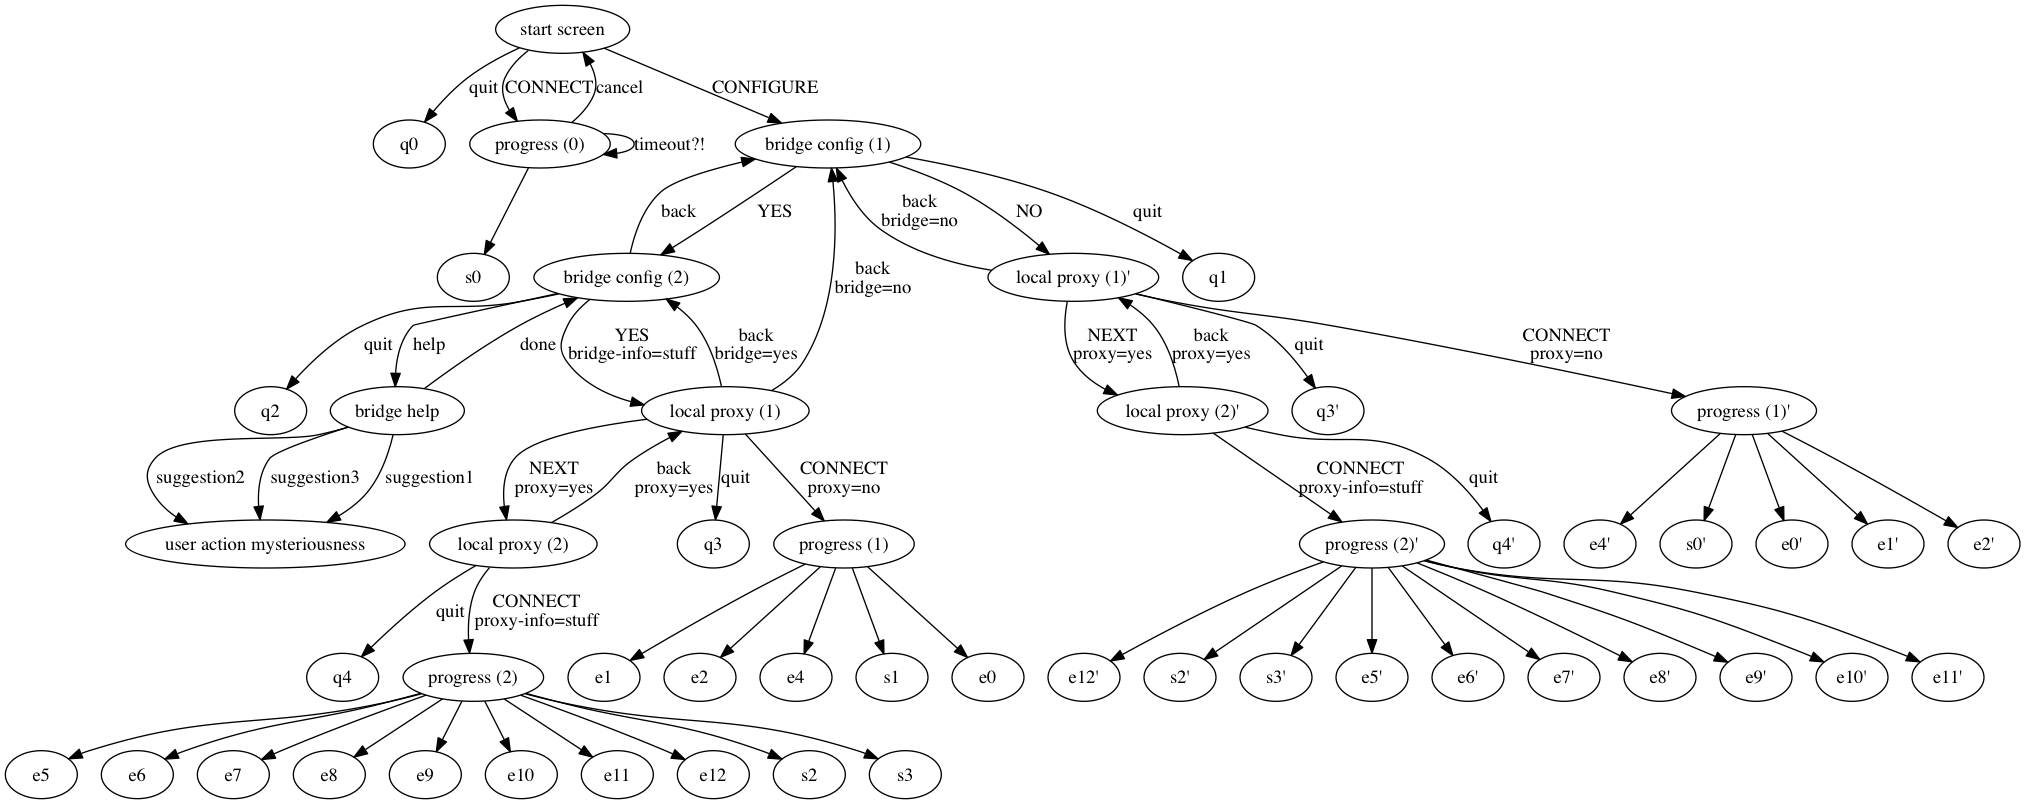
\includegraphics[width=\textwidth]{tor-digraph.png}
\caption{
A digraph illustrating the potential user paths through the interface. Non-leaf nodes are screens in the user interface (start, bridge 1, bridge 2, proxy 1, proxy 2, and progress). Leaf nodes are various end states (quit, success, or error). Transitions between these nodes denote user actions. For details of each end state, see Appendix~\ref{states}. 
}
\label{fig:digraph}
\end{figure*} 

\section{Formative Usability Testing}
\label{sec:qualitative}
This section discusses our small-scale, qualitative usability experiment and resulting user insights. 

\subsection{Recruitment}
We recruited people from Craigslist using the recruitment text in Appendix~\ref{qualitative-recruitment}, which linked an prescreening survey that collected demographics (Appendix~\ref{qualitative-prescreening}). We pre-screened~\cite{screening} for diversity in gender, age, technical expertise, use of security tools, and familiarity with Tor in a small participant pool. {\color {red} Of our 16 recruited participants, 53.3\% were male. Ages ranged from 20 to~62 years ($\mu = 24.5$, $\sigma = 12.6$). 93.3\% of our participants had college education.} We took participants' self-reported familiarity with technical terms use of security tools with skepticism (Appendix~\ref{prescreening-responses}). We verified their self-reported familiarity with Tor Browser in-person, and found that 4 used it, 5 heard of it but not used it, and the remaining 8 never heard of or used it. The main objective of this question was to identify new users versus infrequent users. We considered participants who had never heard of Tor or have only heard of Tor to be new users and those who have used Tor to be previous users. 

We distributed participants evenly across experimental conditions:  5~in E1, 5~in E2, and 6~in E3. Although there is variation in gender, age, ``technical expertise,'' and ``use of security tools'' in each experimental condition, we ensured each condition had a participant who used Tor Browser before. 

\subsection{Setup} 
We ran the experiment in a meeting room in <redacted building> at <redacted university>. The room had a desk and chair, where a monitor, keyboard, and a Windows 8 computer were set up. On a clean computer, we manually downloaded and installed the necessary software for the experiment: Tor Browser 5.0.3 for testing, Chrome, Firefox, and Internet Explorer to allow users to browse the Internet on a another browser of their choice, and VLC to record the screen during the experiment. Before each participant entered the room, we ran a script on the computer that
set up one of the three simulated environments (E1, E2, or E3) and started the recording the computer screen.  

\subsection{Procedure}
Three researchers ran the formative usability testing, with each session having at least two researchers.  
Before the experiment began, each participant was verbally informed of the purpose of the 
study, what data was collected, and any associated risks. If they wished to participate,
they were informed again in writing and consented by signing the document. To be thorough, 
we clarified verbally that they could stop at any time during the experiment with no negative consequences. 

The experiment formally began by informing the participant of the simulated censorship environment (Appendix~\ref{qualitative-script}). This purpose of this introduction was to ensure that the main task
was to connect to Tor, rather than figuring out if they needed to connect to Tor. 
We instructed them to visit a blocked and unblocked website
in a non-Tor browser to clarify that the Internet was functioning as expected. 
We then told them to use Tor Browser to visit a censored site and pointed out 
the respective shortcut on their desktop.

We then asked them to complete a worksheet (Appendix~\ref{participant-worksheet}) that 
required answers from one blocked website (Wikipedia) and one non-blocked website (CNN).
The worksheet did not specify which website was censored. 
We chose these websites because they are popular websites and that their likely familiarity 
would make the task seem less intimidating. 

Participants were given 45 minutes to complete their worksheet. 
After instructions, the researchers left and watched a live feed of the participants' screen in another room to minimize interactions.

After participants completed the browsing tasks (or ran out of time),
we asked them standard interview questions about their experience (Appendix~\ref{interview-questions}) and took notes of their responses. We then followed up with participant-specific questions to verify any hypotheses   we had from observation (e.g. ``the participant was selecting bridges at random''). We paid each participant~\$30 for their time. 

\subsection{Results} 
We give a summary of what our participants did below. We watched the screen recording to summarize their actions and referred to their interviews for insight into why they took specific actions. 

%E1: P2, P3, P4, P9, P10
%E2: P7, P8, P11, P12, P13
%E3: P1, P5, P6, P14, P15, P16

%TODO: re-watch the videos and get the exact times. 
%https://github.com/lindanlee/PETS2017-paper/tree/master/sessions/pre/videos

In E1, any connection to Tor worked. Configuring bridges and proxies were optional.  
Participants in E1 were able to connect to Tor, but most were unsure if their actions were correct. Three of the five participants unnecessarily used bridges. 
Observations in E1: 

%P9 (regular): E1 (0:39; 4:49 to 5:28)
\pquote{P1 (new user, direct, 0:39)}{They connected directly.}

%P2(regular): E1 (1:20, 0:22 to 1:42) 
\pquote{P2 (new user, direct, 1:20)}{They spent time reading the text on the start screen, and connected directly because they were intimidated by the other option.}

%P3(regular): E1 (N/A; 5:47 to 6:26) 
\pquote{P3 (new user, obfs3, 1:39)}{They connected with the recommended bridge. They were also going to use a proxy, but decided not to when they saw the proxy input fields.}

%P4(regular): E1 (8:56, 7:22 to 16:18)
\pquote{P4 (new user, obfs4, 8:56)}{They chose the recommended bridge and then tried to configure a proxy. After not being able to fill out the proxy input fields, they start over and connected using an obfs4 bridge. Note that they didn't try connecting with the obfs3 bridge, which would have worked.}

%P10 (has used Tor before): E1 (1:02; 0:13 to 1:15)
\pquote{P5 (previous Tor user, obfs3, 1:02)}{They connected using the recommended bridge.}

In E2, a bridge was required to connect, but any bridge worked. Configuring a proxy was optional.
Participants in E2 {\it eventually} connected using the recommended bridge, but spent a fair bit of time waiting for direct connections to fail and unsuccessfully configuring proxies. 
Observations in E2: 

%P7 (heard of Tor): E2 (4:04; 0:29 to 4:33) 
\pquote{P6 (new user, obfs3, 4:04)}{They tried connecting directly and gave up after minutes of waiting. Then, they connected using the recommended bridge.}

%P13 (regular): E2 (7:48; 0:34 to 9:22) 
\pquote{P7 (new user, obfs3, 9:22)}{They tried connecting directly. They restarted Tor Launcher and tried another direct connection---and repeated this two more times. On the fourth restart, they tried to configure a proxy, but gave up. On the fifth restart, they connected using the recommended bridge.}

%P12 (regular): E2 (10:40; 0:46 to 11:26)
\pquote{P8 (new user, direct, 10:40)}{They tried connecting directly. They then looked at proxy settings, gave up, and tried connecting directly again. Then, they tried to configure a proxy, and gave up. They tried a direct connection again, which worked. E2 required a bridge to connect, but new public relays came online after we ran our firewall rules and they were able to connect using those new relays.}

%P11 (used Tor before): E2 (~3:00; 1:05 to 5:13)
\pquote{P9 (previous Tor user, obfs3, 4:08)}{They tried connecting directly. Then, they answered no to both bridge and proxy questions, and effectively tried another direct connection. After that, they connect using the recommended bridge.}

%P8 (used Tor): E2 (clock drift mission impossible, 1:38 to 7:20) 
\pquote{P10 (previous Tor user, failed to connect)}{They tried a direct connection. Then, they tried a connection with the recommended bridge, which should have worked. However, our setup experienced a clock drift. Tor does not allow connections with bad clocks. They spent the rest of their time trying different bridges and proxies in vain (Figure~\ref{fig:proxy-attempt}).}

In E3, a bridge was required to connect, but only meek and custom bridges worked. Configuring a proxy was optional.
Participants in E3 struggled. Three failed to connect. Of the three that connected, one brute forced options until something worked (P14), another did not understand what they did (P15), and the third used a custom bridge after being convinced meek bridges were not working (P16).
Observations in E3: 

\begin{figure}[t]
\centering
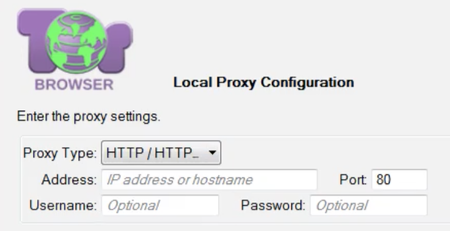
\includegraphics[width=0.5\textwidth]{P8-proxy-attempt.png}
\caption{
Proxies were not necessary to connect to Tor, but many spent time trying to configure one when they couldn't connect. None succeeded. Here, we show P10's unsuccessful attempt. 
}
\label{fig:proxy-attempt}
\end{figure}

%P14 (regular): E3 FAIL
\pquote{P11 (new user, failed to connect)}{They tried connecting directly, and then with the recommended bridge. Then, they retried connecting directly and retried connecting using the recommended bridge. After that, the participant spent the rest of their time trying to configure a proxy and retrying connections with the recommended bridge.}

%P15 (regular): E3 FAIL
\pquote{P12 (new user, failed to connect)}{They tried connecting with the recommended bridge. They decided that they need a proxy along with the recommended bridge, and spent the rest of their time trying to configure a proxy.}

%P16: E3 (regular) FAIL (why did obfs3 work the first time? It shouldn't have!) 
\pquote{P13 (new user, failed to connect)}{They tried connecting directly, and then with the recommended bridge. They retried connecting with the recommended bridge. When that didn't work, they tried to configure a proxy. Then, they gave up and tried using other browsers to complete the task.}

%P6 (heard of Tor): E3 (26:48; 0:18 to 27:06) 
\pquote{P14 (new user, meek-google, 26:48)}{They tried a direct connection by answering no to bridge and proxy questions. After waiting a while, they canceled the connection and tried connecting with the recommended bridge. They retried connecting with the recommended bridge two more times, then tried to connect with a flashproxy bridge, an obfs4 bridge, a scramblesuit bridge. After retrying the recommended bridge again, they made a connection using a meek-google bridge.}

%P1 (heard of tor before): E3 (~7:31, 0:51 to 8:22) 
\pquote{P15 (new user, meek-azure, 7:31)}{They tried connecting directly, and then with the recommended bridge. After that, they tried a connection using a meek-azure bridge, but gave up after before it could connect. They went back to the start screen and clicked connect, which made a connection using meek-azure bridge. The participant thought they made a direct connection, but the connect button used settings toggled in the bridge and proxy screens in the interface.}

%P5 (has used tor before): E3 (22:06; 0:00 to 22:06)
\pquote{P16 (previous Tor user, custom bridge, 22:06)}{They tried and retried connecting directly, then they tried connecting with the recommended bridge. After briefly looking at error messages the system log, they retried connecting directly two more times. After looking up proxy settings, they tried connecting with a meek-google bridge, but gave up before it could connect. They made a connection with the custom bridge by following the instructions from the bridge help button (they created a throwaway email account, emailed the bridge responder with poor syntax and did not get a response, emailed the bridge responder again with correct syntax and got a response, and then typed in the bridge information into the custom bridge field).}

We hope that these participant summaries give some insight into how users may currently struggle with the Tor Launcher interface. 

\subsection{Pain Points in Tor Launcher} 
\label{sec:pain-points}
We talk about the main challenges our participants faced during the experiment. 
Quotations were transcribed live during the follow-up interview.

Participants found the interface confusing, and were often intimidated by the tasks they were asked to do. 

%P8 in the repo, P10 in the paper
\pquote{P10}{``I have no clue what's the difference between flashproxy, fte, etc. And why do I need a custom bridge if there are options built in?''}

%P3 in the repo, P3 in the paper
\pquote{P3}{``The vocabulary is really challenging, for someone not doing IT work.''}

Participants were unsure of what to do, and often configured bridges and proxies when they did not need to.  

%P15 in the repo, but P12 in the paper
\pquote{P15}{``I didn't know if this computer had any proxy information. I wasn't able to find it if it did.''}

The progress bar had system dependencies that made it update oddly. If progress bar reached a 90\% and failed, the progress bar will remain at 0\% on the next attempt until the progress surpassed 90\%. Many assumed that their subsequent attempts were wrong because of this.

%P1 in the repo, P15 in the paper
\pquote{P15}{``It was hard to figure out if the progress bar wasn't moving because the connection was censored, or if it was just slow.''}

We think users in the wild may also face these challenges, and that changes should be made to mitigate them. We show our attempt in the next section. 

\section{A Design Iteration}
\label{sec:design} 
This section discusses how we converted our formative usability testing observations into design changes. 

\subsection{Procedure} 
Three researchers agreed on security and usability design principles. 
We then rewatched screen capture videos and read interview transcriptions to brainstorm design changes. We provided the security and usability design principles, screen capture videos, interview transcriptions, and our suggested changes to a user interface designer, who iteratively redesigned the interface with our feedback and user interface best practices in mind. Figure~\ref{fig:new-interface} shows our redesign of the interface. 

\begin{figure*}
\centering
\begin{subfigure}[b]{0.35\textwidth}
	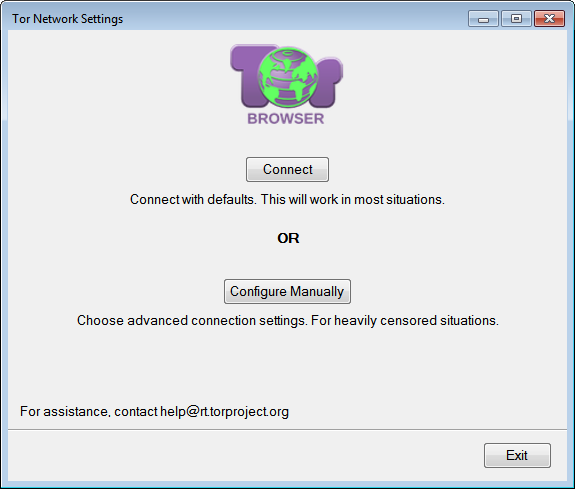
\includegraphics[width=\textwidth]{screenshots/NEW-first.png}
	\caption{The first screen. We reduced the text on the screen and clarified that configuration is for heavily censored environments.}
	\label{fig:new-first}
\end{subfigure}
~~~~~~~~~~
\begin{subfigure}[b]{0.35\textwidth}
	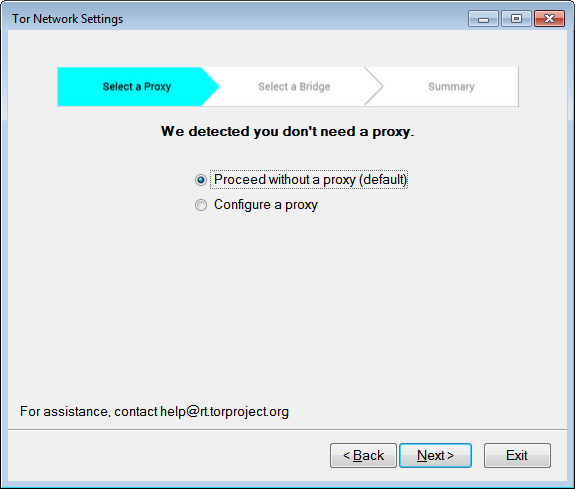
\includegraphics[width=\textwidth]{screenshots/NEW-proxyYES.png}
	\caption{The interface detects the need for a proxy. Proxy fields (same as ones in Figure \ref{fig:old-proxy-yes} are hidden until you click``configure.''}
	\label{fig:new-proxy}
\end{subfigure}
\begin{subfigure}[b]{0.35\textwidth}
	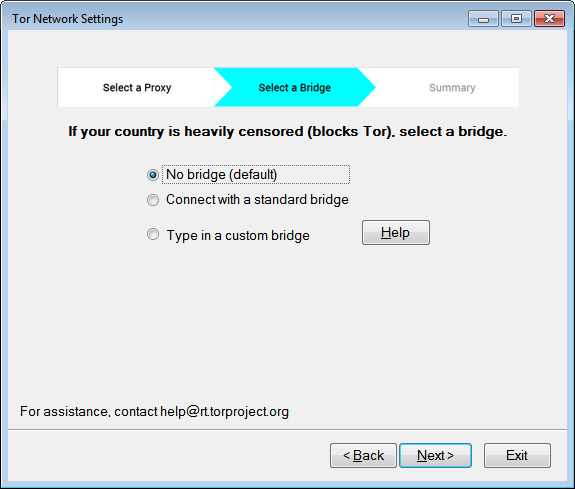
\includegraphics[width=\textwidth]{screenshots/NEW-bridgeSettings.png}
	\caption{There is only one bridge screen now. The default is to connect without one.}
	\label{fig:new-nobridge}
\end{subfigure}
~~~~~~~~~~
\begin{subfigure}[b]{0.35\textwidth}
	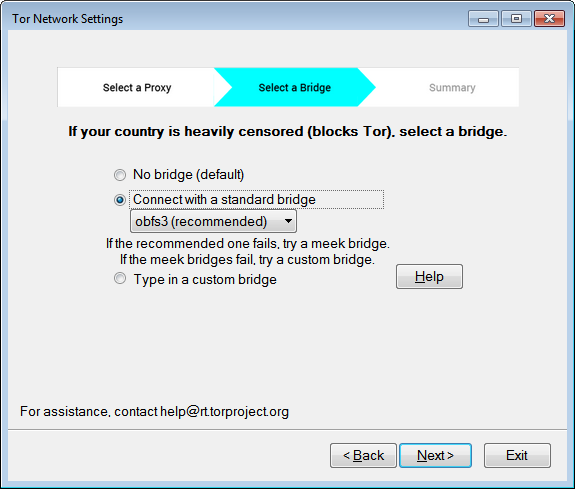
\includegraphics[width=\textwidth]{screenshots/NEW-bridgeSettings-default.png}
	\caption{We give short instructions on when to use a bridge. Users can configure one here.}
	\label{fig:new-bridge}
\end{subfigure}
\begin{subfigure}[b]{0.35\textwidth}
	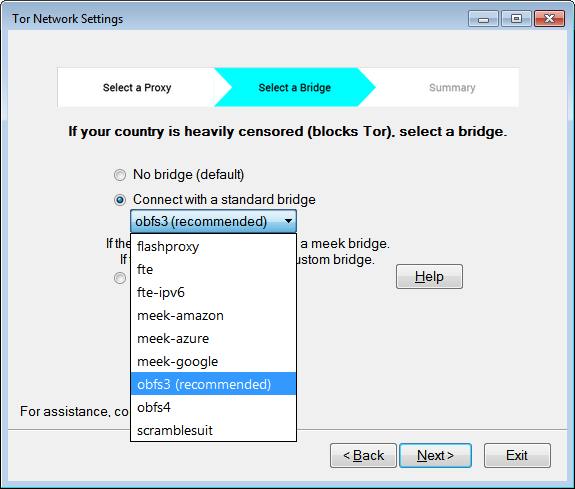
\includegraphics[width=\textwidth]{screenshots/NEW-bridgeSettings-combobox.png}
	\caption{The transports selections are the same.}
	\label{fig:new-bridge-combobox}
\end{subfigure}
~~~~~~~~~~
\begin{subfigure}[b]{0.35\textwidth}
	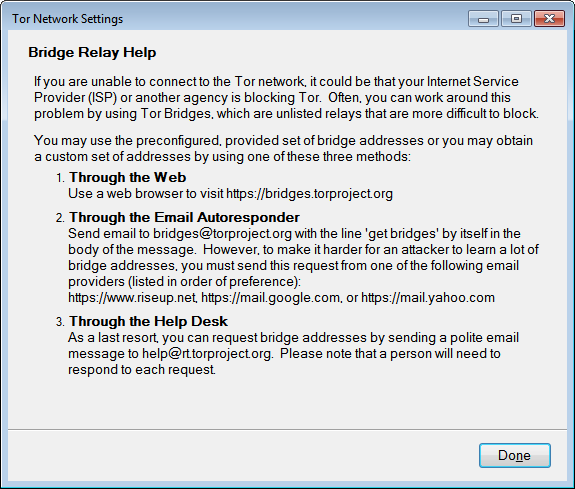
\includegraphics[width=\textwidth]{screenshots/NEW-bridgeHelp.png}
	\caption{These instructions are also the same.}
	\label{fig:new-bridge-help}
\end{subfigure}
\begin{subfigure}[b]{0.35\textwidth}
	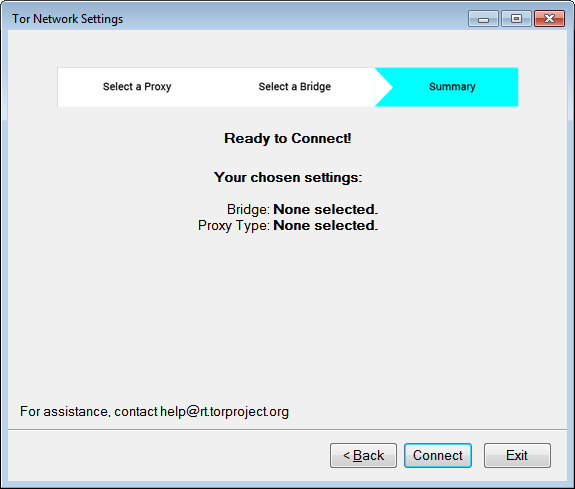
\includegraphics[width=\textwidth]{screenshots/NEW-summary.png}
	\caption{This screen summarized how they would connect to Tor. There is more information if bridges and proxies are configured.}
	\label{fig:new-summary}
\end{subfigure}
~~~~~~~~~~
\begin{subfigure}[b]{0.35\textwidth}
	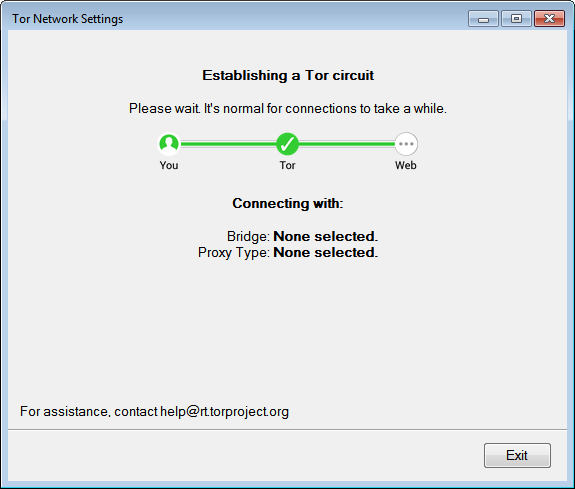
\includegraphics[width=\textwidth]{screenshots/NEW-progress.png}
	\caption{A checkpoint progress bar with connection information. There are more checkpoints if bridges and proxies are configured.}
	\label{fig:new-progress}
\end{subfigure}
\caption{
A redesigned version of the Tor Browser 5.0.3 Tor Launcher GUI. Screens are in the order that they appear. 
}
\label{fig:new-interface}
\end{figure*} 

\subsection{Design Principles} 
The interface currently favors a guided manual configuration over an automated configuration with network probing. Our redesign preserves this approach and has no user-dependent inputs, no network-dependent inputs, and minimal information leaks.

In addition to addressing the pain points we discovered through our formative usability testing (Section~\ref{sec:pain-points}), we aimed to follow usability best practices by minimizing work, giving targeted feedback, and helping users build an understanding of the system.

\subsection{Changes Made} 
We made these changes for a more usable interface. \\

\noindent To minimize work: 
\begin{itemize}
\item We eliminated technical questions, resulting in less tasks and interface screens. 
\item We simulated auto-detection for proxies, telling users that they did not need a proxy. This is feasible to do with a local scan (no information leaked). 
\item We labeled the configure button as an option for users in heavily censored environments.
\item We gave advice on choosing transports, telling users to try a meek bridge if obfs3 does not work.
\end{itemize} 

To give targeted feedback: 
\begin{itemize}
\item We fixed the progress bar so that it reflects the current progress on subsequent attempts. 
\item We switched added indicators to the progress bar to show the progress of bridges and proxies. 
\item We told users what to try next on errors (i.e. choose a different bridge, try a without a proxy). 
\end{itemize}

To build an understanding of the system:
\begin{itemize}
\item We added a summary screen displays the current bridge and proxy settings for system visibility. 
\item We switched proxy and bridge screens to put them in a topologically sequential order (Figure~\ref{fig:topology}).
\end{itemize}

Figure~\ref{fig:new-interface} shows the resulting interface.  Figure~\ref{fig:old-interface} shows the unchanged version. 

\section{Summative Usability Testing}
\label{sec:quantitative}
This section discusses our large-scale quantitative usability experiment and resulting user measurements. 

\subsection{Recruitment}
We recruited  people using the recruitment text in Appendix~\ref{quantitative-recruitment}. We recruited 65 participants from Craigslist and 59 participants from the <redacted lab> participant pool. <Redacted lab> encouraged the use of their participant pool, but we bargained to recruit participants from Craigslist to ensure a diverse set of participants. Although the <redacted lab>'s participant pool is not limited to students and staff from <redacted institution>, it was estimated that a large majority were. 

{\color {red} Of our recruited 124 participants, 56.8\% were male. Ages ranged from 18 to~68 years ($\mu = 28.9$, $\sigma = 12$). 56.8\% were male. 84.8\% of our participants had a college education.} We distributed participants evenly across experimental condition, about 20 in each interface and environment combination. Although there is variation in gender and age in each experimental condition, we ensured each condition had about half Craigslist recruited participants and half <redacted lab>  pool participants. 

\subsection{Setup}
We ran our experiment at <redacted lab>, an experimental social science laboratory for behavioral experiments. The testing room had 36 workstations with identical Windows~7 laptops. Side panels at each workstation to discouraged participants from looking at other participants' screens. 
%Xlab~\cite{xlab}, the Experimental Social Science Laboratory at the University of California, Berkeley. 
The computers at <Redacted lab> use a system restore software to revert computers to a clean version at the beginning of each session. 

Before each session, we ran a script that downloaded the necessary software, set up one of the three simulated environments (E1, E2, or E3), and downloaded the original Tor Browser 5.0.3 or a modified version of Tor Browser 5.0.3 that contained our design changes (OLD or NEW), and start the video recording. In contrast to the previous test, we installed an instrumented versions of Tor Browser 5.0.3. The instrumentation logged user interactions, such as window transitions, mouse clicks, and menu selections. Similarly to the previous test, we installed Chrome, Firefox, and Internet Explorer to allow users to browser the Internet on a browser of their choice and VLC to record the screen during the experiment. Each computer was manually assigned one of the six interface--environment combinations in a way that evenly distributed experimental conditions throughout the room and assigned an equal number of participants to each experimental condition.

\subsection{Procedure}
Participants were assigned to a computer at random, which effectively assigned them to a simulated censorship environment combination at random. Before the experiment began, participants were verbally informed of the purpose of the study, what data was collected, and any associated risks. If they wished to participate, they were informed again in writing and consented by signing the document. To be thorough, we clarified that they could stop at any time during the experiment with no negative consequences. 

The experiment formally began by informing participants of the simulated censorship environment, giving them their worksheet, and informing them that Tor browser is necessary to circumvent censorship (Appendix~\ref{quantitative-script}). This time, the worksheet only asks users to visit one blocked website (Wikipedia) and explicitly reminds users to use Tor to do so. Before participants started their tasks, we reminded them that their screens are being recorded so they should not log into anything that shows personal information. We gave users a chance to ask any questions about the experiment or task. 

Participants were given 40 minutes to complete the task. After instructions, researchers maintained minimal interactions with the participants, only answering logistical questions. Afterward, we administered an exit survey to collect demographics (Appendix~\ref{quantitative-exit-survey}). We paid each participant \$30 for their time. 

\subsection{Results} 
124 people participated in our experiment, but we used data from 114. We filtered participants who made errors in completing the consent form, did not understand the task, or did not interact with the instrumented interface. In this section, we use OLD to refer to the deployed Tor Browser 5.0.3 Tor Launcher GUI (Figure~\ref{fig:old-interface}) and NEW to refer to our redesigned version (Figure~\ref{fig:new-interface}). Table~\ref{table:participant-summary} gives an overview of the results and Figure~\ref{fig:all-participant-edges} summarizes all participants' paths during the experiment.

\begin{table}[t]
\centering
\begin{tabular}{l r r r r r}
& \multicolumn{2}{r}{completion rate} & \multicolumn{1}{r}{connection} & \multicolumn{1}{r}{configuration} \\
& \multicolumn{2}{r}{(at 40 minutes)} & \multicolumn{1}{r}{time (med)} & \multicolumn{1}{r}{time (med)} \\
\noalign{\hrule}
E1-NEW & 19/19 & 100\% & 0:20 & 0:06 \\
E1-OLD & 19/19 & 100\% & 1:01 & 0:24 \\
E2-NEW & 18/18 & 100\% & 3:22 & 0:40 \\
E2-OLD & 16/19 & 84\% & 5:00 & 2:04 \\
E3-NEW & 13/19 & 68\% & 20:25 & 1:56 \\
E3-OLD & 10/20 & 50\% & 40:08 & 9:09 \\
\end{tabular}
\caption{
An overview of the results of the experiment. Those who
failed to connect were assigned the maximum time of 40:08.
}
\label{table:participant-summary}
\end{table}

\label{all-participant-edges} 
\begin{figure*}
\centering
% This is a manually edited version of the automatically generated
% all-participant-edges graphic. It is edited to have better scale labels for
% the treatments.
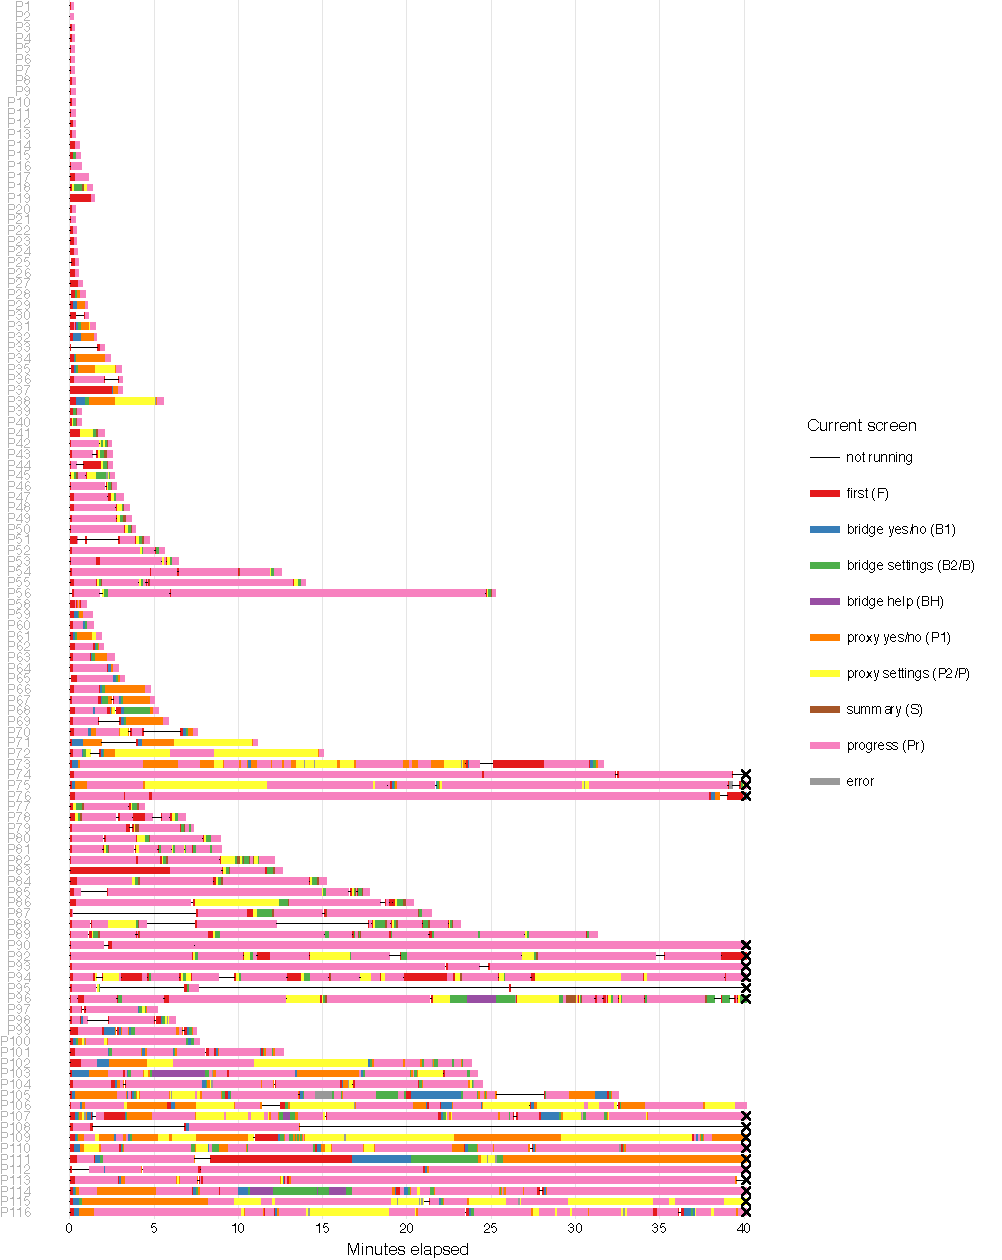
\includegraphics{all-participant-edges}
\caption{
A summary of our valid participants' paths through the interface.
The length of the bars show the total time taken to complete the task,
except for those we cut off after approximately 40 minutes.
Different colors indicate which screen they were on during the experiment.
The ``not running'' times are those when Tor Launcher was closed (
i.e. searching for help in another browser, restarting the application, etc.).
}
\label{fig:all-participant-edges}
\end{figure*}

\subsubsection{Completion Rate} 

%table
\begin{table}[t]
\centering
% Do not edit this file. Edit attempts.R instead.
\begin{tabular}{r c c c c c c}
& \rotatebox{90}{E1-NEW} & \rotatebox{90}{E1-OLD} & \rotatebox{90}{E2-NEW} & \rotatebox{90}{E2-OLD} & \rotatebox{90}{E3-NEW} & \rotatebox{90}{E3-OLD} \\
no bridge, no proxy & 17 & 13 &  &  &  &  \\
obfs3, no proxy & 2 & 6 & 18 & 16 &  &  \\
meek-amazon, no proxy &  &  &  &  & 7 & 4 \\
meek-google, no proxy &  &  &  &  & 5 & 4 \\
meek-azure, no proxy &  &  &  &  & 1 & 1 \\
no bridge, 3rd-party proxy &  &  &  &  &  & 1 \\
DNF (did not finish) &  &  &  & 3 & 6 & 10 \\
\end{tabular}

\caption{
Network components that led to the first successful bootstrap
in each condition.
Most successful E1 participants used a direct connection,
but a few optionally used an obfs3 bridge.
All successful E2 participants used 
an obfs3 bridge (the recommended option)---none used 
flashproxy, fte, fte-ipv6, obfs4, or scramblesuit bridges to connect. 
Most successful E3 participants
used a meek bridges, disfavoring meek-azure.
One E3 participant succeeded in an unexpected way
by using an open proxy and configuring it to bypass our 
simulated environment.
}
\label{tab:attempts-bridge-proxy}
\end{table}

%overview
Completion rate was defined as the percentage of users that eventually connected to Tor. Table~\ref{table:participant-summary} summarizes the completion rates and Table~\ref{tab:attempts-bridge-proxy} shows the configuration for users' first successful connection. We only considered the first successful configuration, as some curious participants tried others after completing their task. 

% failure observations
17\% (19 of 114) of participants were not able to successfully connect to Tor. Five (P73, P75, P89, P91, P106, P110) tried a direct connection. When that failed, they assumed there was something wrong with their computer, network settings, or the Tor network and never tried to configure bridges or proxies. Five (P74, P92, P105, P107, P113) users who need a bridge assumed that they needed a proxy to connect to Tor. We believe this may be due to the fact that the OLD interface defaults to showing users the proxy page (because it is the one before the progress screen) when a connection fails. Five (P90, P93, P108, P111, P114) users who needed a meek or custom bridge tried the suggested bridge (obfs3), but didn't know what to do when that failed. Two (P94, P109) users who needed a meek or custom bridge tried to get custom bridges but failed to format their email content correctly to get a response from the bridges autoresponder. We suspect that they would have succeeded if they had gotten a response. 

%success rate and version
Our interface changes did {\it not} have a significant impact on completion rates (Pearson's Chi-squared; $X^2 = 0.0126$, $df = 2$, $p = 0.994$). That is, the slight differences in completion rates between E1-NEW vs E1-OLD, E2-NEW vs E2-OLD and E3-NEW vs E3-OLD are likely due to random chance.

\subsubsection{Connection time} 
Connection time is the time from Tor Browser startup to the first successful Tor bootstrap. Non-finishing participants are assigned the maximum experiment time of 40:08. Table~\ref{table:participant-summary} summarizes the median times while Figure~\ref{fig:time_to_success_clamped} shows their distribution. Figure~\ref{fig:time_to_success_ecdf} shows the cumulative success rates over time. 

%time observations (how long people took)
The simulated censorship environment, and therefore, the difficulty of the configuration, was the most determining factor for connection time (Kruskal--Wallis $\chi^2 = 80.5$, $\mbox{df} = 2$, $p < 10^{-15}$). Participants in E2 took longer to connect than participants in E1, and participants in E3 took the longest to connect.

%time to success and version
Our interface changes had a significant impact in reducing connection time (one-tailed Mann--Whitney; $ Z = -1.84$, $p = 0.0328$, $r= 0.172$). That is, the differences in mean connection times in E1-NEW vs E1-OLD and E2-NEW vs E2-OLD and E3-NEW vs E3-OLD is likely not due to random chance. We used a one-tailed Mann--Whitney test because the distribution of completion times were 1) right-censored at 40 minutes (experiment duration) and 2) non-normal and heavily right tailed (failures were assigned a time of 40 minutes). 

\begin{figure}[t]
\centering
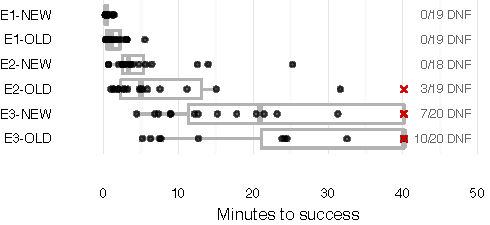
\includegraphics{time_to_success_clamped}
\caption{
The dots show the raw connection times,
while the boxplots show the medians and interquartile ranges.
The ``DNF'' (did not finish) numbers at the right show how many of participants 
did not finish, who were assigned the maximum time of 40:08.
}
\label{fig:time_to_success_clamped}
\end{figure}

\begin{figure}[t]
\centering
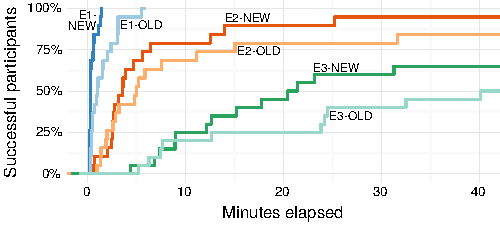
\includegraphics{time_to_success_ecdf}
../experiment/processing/time_to_success_ecdf.tex
\caption{
Cumulative success rates over time, shown continuously and at discrete times we found interesting.
For the purposes of plotting the cumulative distribution, those who did not finish were assigned
an arbitrarily high number greater than 40 minutes. 
Notice that the longer the time went on, participants were less likely to succeed. 
At 1.5 minutes, every E1-NEW participant finished,
but only 58\% of E1-OLD had finished by that time.  
At 10 minutes, most participants in E2 had finished. 
}
\label{fig:time_to_success_ecdf}
\end{figure}


\subsubsection{Configuration Time} 
Configuration time is the time spent configuring network components, which we define as the completion time minus any time spent on the progress screen. Table~\ref{table:participant-summary} shows the median times and Figure~\ref{fig:time_to_success_active_clamped} shows their distribution. Table~\ref{table:median_time} shows the percentage of time spent on each screen. Note that the time spent configuring bridges and proxies is {\it not} equivalent to the amount of time participants spent trying to connect, which would be the connection time minus the time spent on the progress screen for the last time (time Tor takes to bootstrap after a valid configuration). 

%things to keep in mind
We believe that configuration time is a meaningful metric because 1) bootstrapping can take a couple minutes, which dominates measurements for users do not need much time to configure their connection, such as participants in E1, and 2) some mistakes, such as using a syntactically valid but unusable proxy, generate non-interrupting warnings and let the users wait indefinitely at until they manually cancel the connection to try again. But this is not the most accurate measurement of time spent configuring, since it does not reflect how some participants searched for help in another browser while waiting on the progress screen.

%configuration time and version
Our interface changes had a significant impact in reducing configuration time (one-tailed Mann--Whitney; $Z = -3.28$, $p = 0.000516$, $r = 0.307$). That is, the differences in mean configuration times in E1-NEW vs E1-OLD and E2-NEW vs E2-OLD and E3-NEW vs E3-OLD is likely not due to random chance. We used a one-tailed Mann--Whitney test because the distribution of configuration times were also 1) right-censored and 2) non-normal and heavily right tailed, due to being an artifact of completion time. 

\begin{table}[t]
\centering
\begin{tabular}{l r r r r}
& First & Proxy & Bridge & Progress \\
\noalign{\hrule}
E1-NEW & 28\% & 0\% & 0\% & 60\% \\
E1-OLD & 30\% & 0\% & 0\% & 29\% \\
E2-NEW & 6\% & 5\% & 6\% & 78\% \\
E2-OLD & 7\% & 18\% & 8\% & 45\% \\
E3-NEW & 3\% & 5\% & 5\% & 77\% \\
E3-OLD & 2\% & 12\% & 6\% & 64\% \\
\end{tabular}

\caption{The median percent of time spent on each screen, which is not
necessarily the median absolute time spent on that screen. 
This percentage is computed independently for each screen; that is, a participant who spent the median percent 
of time on one screen may not be the same participant who spent the median percent
of time on other screens.} 
\label{table:median_time}
\end{table}

\begin{figure}[t]
\centering
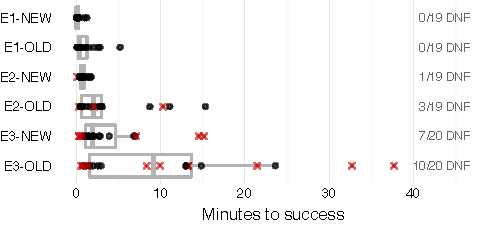
\includegraphics{time_to_success_active_clamped}
\caption{
The dots show the raw active configuration times,
while the boxplots show the medians and interquartile ranges.
Here, non-finishing participants' active time was computed by
subtracting the amount of time spent on the progress screen from the 
their assigned completion time of 40:08.
}
\label{fig:time_to_success_active_clamped}
\end{figure}

\subsection{Usability of Tor Launcher} 
In total, 63\% (72 of 114) of first attempts to connect failed and 79\% (363 of 458) of total attempts to connect failed. 
On average, users who required a bridge took over 3 minutes to connect to Tor, and users who required a meek or custom bridge took over 20 minutes.

Ideally, almost all users should be able to configure the necessary or optional network components and connect to Tor within a few minutes. Neither the Tor Browser's 5.0.3. Tor Launcher GUI or our redesigned Tor Launcher GUI meets this goal.

\section{Recommendations}
\label{sec:recommendations}
We do believe that adopting our design will help save users time when connecting to Tor. But since we did not test our design changes independently, we cannot (and do not) claim the effects each change we made. Therefore, we do not recommend specific changes, but offer some suggestions for Tor Launcher's GUI based on what we learned: \\

\begin{itemize}
\item {\bfseries Hide infrequent options.} Hide the proxy configuration screen and less-used transports. None of our participants connected using flashproxy, fte, fte-ipv6, or scramblesuit transport bridges. 
\item {\bfseries Give advice.} Discourage users from configuring optional components. Add a secondary recommendation for bridges (try meek if obfs3 doesn't work, use meek if you are in Syria) to help users in need. 
\item {\bfseries Minimize work.} Detect if users need a proxy or not. Redirect users to the relevant pages on error (i.e. redirect to the bridge screen the bridge fails).  
\item {\bfseries Provide feedback.} Tell users what to do when a specific error occurs (i.e. try the same connection again, pick another bridge, try without a proxy, etc.).  Show users their bridge and proxy settings before and during connection. Fix the progress bar so that it updates on subsequent connections.
\end{itemize}

We also recommend exploring solutions that leverage automation, user-dependent inputs, or network-dependent inputs. We start this discussion by sharing some of our own ideas in appendix~\ref{alternatives}. 

\section{Limitations}
\label{sec:limitations}
We did not study international users, or the configuration interface in languages other than English. All of our participants were from the United States and instructed to interact with the English version of Tor Browser.

Participants in a laboratory setting may alter their due to their awareness of being observed~\cite{mccarney2007hawthorne}. We are aware that our participants were likely motivated differently compared to real users. We believe that participants were likely overmotivated to connect to Tor because they were being observed and receiving a monetary reward. If true, this makes our results are a conservative estimate of the current usability problems. 

Since the configuration interfaces in simulated environments, we cannot claim how difficult it would be for a user to connect to Tor in a certain country or how much our redesigned interface would help those users.  

Our experiment did not directly test more advanced tasks. Our simulated environments did not require users to configuring a proxy or to get a custom bridge. From observing of user attempts to configure proxies and get custom bridges, we suspect users generally struggle with these tasks but cannot quantify how much they do. 

We only tested interface on Windows machines, which were the machines available at <redacted>. %Xlab.
The configuration interface leverages the native operating system's styling and elements, making the configuration interface on Windows look slightly different from the OS~X or Linux equivalent. Additionally, we acknowledge that participants' unfamiliarity with Windows may have affected our experiment, but we believe that this affected all experimental conditions minorly and equally.  

\section{Related Work}
\label{sec:related} 

{\color {red} 
There have been three published user studies on Tor. Clark et~al.~\cite{clark2007usability} examined various deployment
options for Tor Browser, such as Vidalia, Privoxy, Torbutton, and FoxyProxy, and found that none had satisfactory from a usability. Fabian et~al.~\cite{fabian2010privately} show that Tor's added
latency~\cite{dingledine2009performance} causes users
to be frustrated, cancel requests, and prevents user adoption. 
Norcie et~al.~\cite{norcie2012eliminating} found found that 
64\% of users are unable to continue with installation or browsing at least once due to difficulties.

We do not know of any published usability evaluations of
Tor Browser since the release of the 3.5 series in 2013, which introduced radical UI changes~\cite{torbrowser-35}.
The most recent effort is an unpublished pilot study by Lee and Fifield~\cite{uxsprint} 
that tested the downloading, installation, and browsing tasks in Tor Browser.  This study uncovered a number of issues~\cite{uxsprint2015-tickets},
some of which influenced changes in Tor Browser version~4.5 and later.

Previous user studies have considered the whole browsing experience,
without focusing on specific features in isolation.
Our study focuses on 
the browser's configuration interface, which guides users through setting up components required to circumvent censorship. 
%for color red
}

\section{Conclusion} 
\label{sec:conclusion}
The Tor Launcher GUI allows most users to connect to the Tor network, provided that the user's connection does not require a proxy or a non-default bridge. User observation showed that participants were intimidated of the tasks, unsure of what to do, and likely to get stuck configuring proxies that they did not need. User testing showed that most people take more than 10 minutes to connect to Tor if they need to use bridges. 

%proof that user testing is important and general advice to for more research on Tor
We encourage usability testing for Tor Browser and other Tor applications because it provides user insight for products without user interaction data. Tor Browser version~4.5 incorporated changes to Tor Launcher based on our work <redacted Tor blog post here; it was authored by one of the authors of this paper>. We also talked to Tor developers about ways to automate the bootstrapping process to Tor. 

\section {Experiment Artifacts} 
Due to space constraints, we could not include many of our experiment artifacts. This includes the experiment setup and teardown code, firewall rules that simulated censorship environments, interview transcriptions from the formative user study, logs from our instrumented configuration interfaces, and videos of users attempting to connect to Tor through the configuration interface. We urge you to check out the project repository: \\

\noindent <redacted url>
%\noindent \url{https://github.com/lindanlee/circumvention-ux-tor}

\section {Acknowledgments}
Many generous people helped us along the way. <Redacted> assisted with testing our setup and teardown scripts, offered recruitment services, and allowed us to run experiments after <redacted lab>'s hours. <Redacted> and <redacted> were instrumental during the design process, as they helped me iterate through many not-so-great ideas.  <Redacted>, and <redacted> provided me with insider insight into the design decisions made at Tor.
% Rowilma del Castillo. Nima Fatemi and Isabela Bagueros.  Georg Koppen and the Tor UX team.

\bibliographystyle{abbrv}
\bibliography{pets2017-paper}

\appendix

\section{Success and Error States in Tor Launcher 5.0.3} 
\label{states} 
An exhaustive list of Tor Launcher 5.0.3's end states corresponding to Figure~\ref{fig:digraph}. End states such as e\# and e\#' are equivalent, but e\#' uses a bridge while e\# does not. This was generated during the inspection process.\\

\noindent success states: 
\begin{itemize}
\item s0: no bridge no proxy
\item s1: valid bridge, no proxy
\item s2: valid bridge and valid proxy (blank port)
\item s3: valid bridge and valid proxy (specified port)
\end{itemize}

error states:
\begin{itemize} 
\item e0: custom bridge: field left blank
\item e1: custom bridge: syntax error
\item e2: custom bridge: invalid address
\item e3: hardcoded bridge blocked
\item e4: custom bridge blocked
\item e5: proxy type is not selected
\item e6: proxy: ip address left blank
\item e7: proxy: syntax error
\item e8: proxy: invalid ip address, blank port
\item e9: proxy: invalid ip address, good port
\item e10: proxy: invalid ip address, bad port
\item e11: proxy: valid ip address, bad port
\item e12: proxy: valid ip address, blank port
\end{itemize} 

The same input can lead to different end states. Tor Launcher will connect to a proxy successfully with the port left blank if the proxy uses port 80 (s2) but will not if the proxy uses another port (e12). 

\section{Qualitative User Study Recruitment Posting} 
\label{qualitative-recruitment}
We are recruiting participants for an in-person research study at <redacted>. %the University of California, Berkeley. 
You will need to come in to our lab and perform tasks on a computer for an hour or less. You will be compensated \$30 for participating. 
No special knowledge and no technical experience is required. If you are interested, fill out the survey at \textit{<survey link>}. 

\section{Qualitative User Study Prescreening Survey} 
\label{qualitative-prescreening}
We are recruiting participants for an in-person research study at the <redacted>. %University of California, Berkeley. 
You will need to come in to our lab and perform tasks on a computer for an hour or less. You will be compensated \$30 for participating. No special knowledge and no technical experience is required.\\

\begin{enumerate}
\item{Please select when you are available. We will assign you an hour experiment time slot during one of those times.}
\item{I am able to provide my own transportation to the <redacted> %University of California, Berkeley 
campus.}
\item{Thank you for your interest! Please provide an email address where we can contact you to share more logistical details.}
\item{we are looking for a very small number of participants, so unfortunately, we may not be able to accommodate everyone who applies. Would you like us to let you know about future opportunities?}
\item{What is your gender?}
\item{What is your age?}
\item{Please select your highest completed (or current) level of education.}
\item{What is your occupation?} 
\item{Do you speak any languages other than English fluently?}
\item{If you have a personal computer, what kind do you use?}
\item{Which of the following terms have you heard of? \textit{<answer choices: a checkboxlist of the the following terms: malware, proxy services, phishing, SSL, X.511 certificates, Tor>}}
\item{How often do you use the following software or features? \textit{<answer choices: a grid of radio buttons. Software/features (rows): HTTPS on web pages, proxies or other censorship circumvention tools, virtual private networks (VPN), file or whole-disk encryption, anonymity systems (e.g., Tor), email encryption (e.g., PGP), chat or instant messaging encryption, voice communication encryption. Frequency (columns): never, less than once a month, a few times a month, several times a week, daily.>}}
\end{enumerate}
Thank you for filling out this form. You are now done!

{\color {red}
\section{Prescreening Survey Responses}
\label{prescreening-responses}
We asked people how familiar they were with some technical terms and security tools during our prescreening survey for formative usability testing. We show the responses from the participants that we chose. 

\begin{table}[h]
\centering
\begin{tabular}{l r r}
& Familiarity\\
\noalign{\hrule}
Malware & 00/00\\
Proxy services & 00/00\\
Phishing & 00/00\\
SSL & 00/00\\
X.511 certificates & 00/00\\
Tor & 00/00\\
\end{tabular}
\caption{
An overview of the results of the experiment. Those who
failed to connect were assigned the maximum time of 40:08.
}
\label{table:selfreported-tech}
\end{table}

We suspect that participants answered dishonestly in hopes of appearing more technically fluent. We know this because some reported that they were familiar a term that did not exist (x.511 certificates). We inserted this fictional term specifically to detect this. 

\begin{table*}[h]
\centering
\begin{tabular}{l r r r r r}
& \multicolumn{1}{r}{} & \multicolumn{1}{r}{Less than once} & \multicolumn{1}{r}{A few times}& \multicolumn{1}{r}{Several times}& \multicolumn{1}{r}{}\\
& \multicolumn{1}{r}{Never} & \multicolumn{1}{r}{a month} & \multicolumn{1}{r}{a month}& \multicolumn{1}{r}{a week}& \multicolumn{1}{r}{Daily}\\
\noalign{\hrule}
HTTPS on web pages& 00/00 & 00/00 & 00/00 & 00/00 & 00/00 \\
Proxies or censorship circumvention tools & 00/00 & 00/00 & 00/00 & 00/00 & 00/00 \\
Virtual private networks (VPNs) & 00/00 & 00/00 & 00/00 & 00/00 & 00/00 \\
File or disk encryption & 00/00 & 00/00 & 00/00 & 00/00 & 00/00 \\
Anonymity systems (e.g. Tor) & 00/00 & 00/00 & 00/00 & 00/00 & 00/00 \\
Email encryption (e.g. PGP) & 00/00 & 00/00 & 00/00 & 00/00 & 00/00 \\
Instant messaging encryption & 00/00 & 00/00 & 00/00 & 00/00 & 00/00 \\
Voice communication encryption & 00/00 & 00/00 & 00/00 & 00/00 & 00/00 \\
\end{tabular}
\caption{
An overview of the results of the experiment. Those who
failed to connect were assigned the maximum time of 40:08.
}
\label{table:selfreported-software}
\end{table*}

We assume that self-reported use is the upper bound of how many participants have used these security tools.
}

\section{Qualitative User Study Introduction Script} 
\label{qualitative-script} 
Imagine you live in an oppressive country that censors part of the Internet. We have simulated this in the laboratory by blocking certain websites and services.  The purpose of this experiment is to evaluate the use of Tor browser, which is a browser that can circumvent censorship and let you visit blocked websites. Currently, torproject is blocked (you can check this by going to torproject.org on a standard browser, like Firefox, Chrome, or Internet Explorer). 

To circumvent censorship successfully, you will need to set up Tor browser correctly and use it to get to Wikipedia. If you are able to reach the website, then you know that you have successfully circumvented censorship. Fill out the question on the worksheet. This isn't intended to be hard, just write what you see. We want to just check you saw the website. 

Before you start, do you have any questions about what you are asked to do? 

\section{Participant Worksheet Text} 
\label{participant-worksheet}
Imagine you live in an oppressive country that censors part of the Internet. We have simulated this in the laboratory by blocking certain websites and services. The purpose of this experiment is to evaluate the use of Tor browser, which is a browser that can circumvent censorship and let you visit blocked websites. For instance, www.torproject.org is blocked. Check this by going to the site on a standard browser, like Firefox, Chrome, or Internet Explorer. It will fail to load, when you can visit other sites.

To complete this worksheet, you will need to set up Tor browser (on your desktop) correctly and use it to get to blocked site. If you can visit wikipedia, then you know that you have successfully circumvented censorship.

\section{Post-Experiment Standard Interview Questions}
\label{interview-questions}
We asked our participants these questions after they were given time to configure Tor Browser. \\

\begin{enumerate}
\item{Can you talk us through what you did along with what you were thinking at the time?}
\item{What was most challenging part of connecting?}
\item{Were there any unfamiliar terms?}
\item{How did you decide which options to choose?}
\item{What did you think about using Tor?}
\item{What is one change you would recommend?} 
\item{Did you need any additional information?} 
\end{enumerate}  

In addition to these questions, we asked our participants about specific questions based on their observation, usually regarding a specific choice in action, a particular screen they seemed stuck on, and any errors they encountered during the configuration process. 

\section{Quantitative User Recruitment Posting}
\label{quantitative-recruitment}
We are recruiting up to 40 participants for a user study at <redacted>. %UC Berkeley. 
The experiment will involve basic Internet browsing tasks. You are not eligible if you have participated in our previous sessions.\\

\indent Payment: \$30 Amazon gift card\\
\indent Duration: 1 hour \\
\indent Where: <redacted> \\ %Xlab at Hearst Memorial Gymnasium\\

\textit{<list of sessions>}\\

To be eligible, you must be an adult (18 or older). This is to comply with university policies on research. 

If you are interested: 1. Email <redacted> %lnl@berkeley.edu 
with the sessions you are able to attend. We will confirm your participation and assign you a session. 
2. Come to <redacted> %Xlab 
at the appointed time for the experiment.

\section{Quantitative User Study Introduction Script} 
\label{quantitative-script} 
Imagine you live in an oppressive country that censors part of the Internet. We have simulated this in the laboratory by blocking certain websites and services.  The purpose of this experiment is to evaluate the use of Tor browser, which is a browser that can circumvent censorship and let you visit blocked websites. Currently, torproject is blocked (you can check this by going to torproject.org on a standard browser, like Firefox, Chrome, or Internet Explorer). 

To circumvent censorship successfully, you will need to set up Tor browser correctly and use it to get to Wikipedia. Tor is already installed for you. On the desktop, you should see a globe icon that says ``Start Tor Browser.'' If you are able to reach the website, then you know that you have successfully circumvented censorship. Fill out the question on the worksheet. This isn't intended to be hard, just write what you see. We want to just check you saw the website. 

Afterward, we ask you to take a short survey to collect some information about you. The link is also on your worksheet.
We will give you time to complete this task. If you finish early, we ask that you sit at your desk until the remainder of the hour. Since we are recording your screen, we ask that you don't do anything personal afterward, like checking your email.

Before you start, do you have any questions about what you are asked to do? 

\section{Quantitative User Study Exit Survey} 
\label{quantitative-exit-survey}
We'd like to know more about you.  All of your answers will be stored separately from any identifying information in order to protect your confidentiality.

This survey is part of a research project being conducted by the <redacted>. %University of California, Berkeley. 
If you have any questions about your rights or treatment as a research participant in this study, please contact the <redacted>'s %University of California at Berkeley's 
Committee for Protection of Human Subjects at 510-642-7461, or email 
<redacted>. %subjects@berkeley.edu. 
If you agree to participate, please click Next below.\\

\begin{enumerate}
\item{What is your participant ID? (This can be found on the sticker on the left hand corner of the desk you are currently sitting at.)}
\item{What is your gender?}
\item{What is your age?}
\item{Please select your highest completed (or current) level of education}.
\item{What is your current occupation?}  
\end{enumerate}

Thank you for participating in our experiment. You are now done! Please sit at your desk for the remainder of the experiment. Our researchers will formally announce the end of the experiment. 

\section{Alternative Approaches} 
\label{alternatives}
We list some of our ideas:\\
\begin{description}
\item{\bfseries Suggest bridges based on country.} Give users information about which bridges would work in their country. one way to do this is to show a list of countries with a corresponding recommended configuration. This requires developers to maintain a list of suggestions and that the users trust the suggestions. 
\item{\bfseries Ask users about their risk.} If they answer that they are sensitive about having a network adversary possibly know that they are using Tor, direct users to connect to a secret relay that is not publicly associated with Tor, using transport that obfuscates their connection. If users are not sensitive, let them configure their own bridges and proxies. 
\item{\bfseries Ask users if they know what to do.} If they know, offer the option to manually configure bridges and proxies. If they do not know, give suggestions on what to do next or automate the process for them somehow. This requires users to answer honestly to the question and to trust the suggestions given. 
\item{\bfseries Automate naively.} Have the interface automatically try configurations that would most likely work, in order (i.e. a direct connection, then an obfs3 connection without a proxy, then an meek bridge connection with out a proxy). This is what most users would ideally do anyway. However, this method leaks to network eavesdroppers that the user is using Tor without the user's awareness. 
\item {\bfseries Automate naively after users fail.} Let users try to configure bridges and proxies. If they fail, then a network adversary already knows that the user is trying to connect to Tor. At this point, we believe that it is low risk to naively automate configuring bridges and proxies. 
\item{\bfseries Automate in a smart way.} The interface first detects proxy settings and uses them, if any. Then it automatically connects to some secret bridges that will always work, which assign the user an entry relay that works based on their location. This requires having an invincible set of high-bandwidth bridges that work for every single user around the world.  
\end{description}

We believe that these ideas can significantly help users connect to Tor. 


\end{document}
